\section{Unit tests}

\subsection{Eingesetzte Software}

Für die Qualitätssicherung nutzen wir schon seit der Implementierungsphase Jest, um die Funktionalitätr der einzelnen methoden zu teste. Das haben wir zusätzlich mit enzyme ergänzt, womit wir die Funktion gesamter React-Komponenten einfach testen können.

\subsection{Testcoverage}
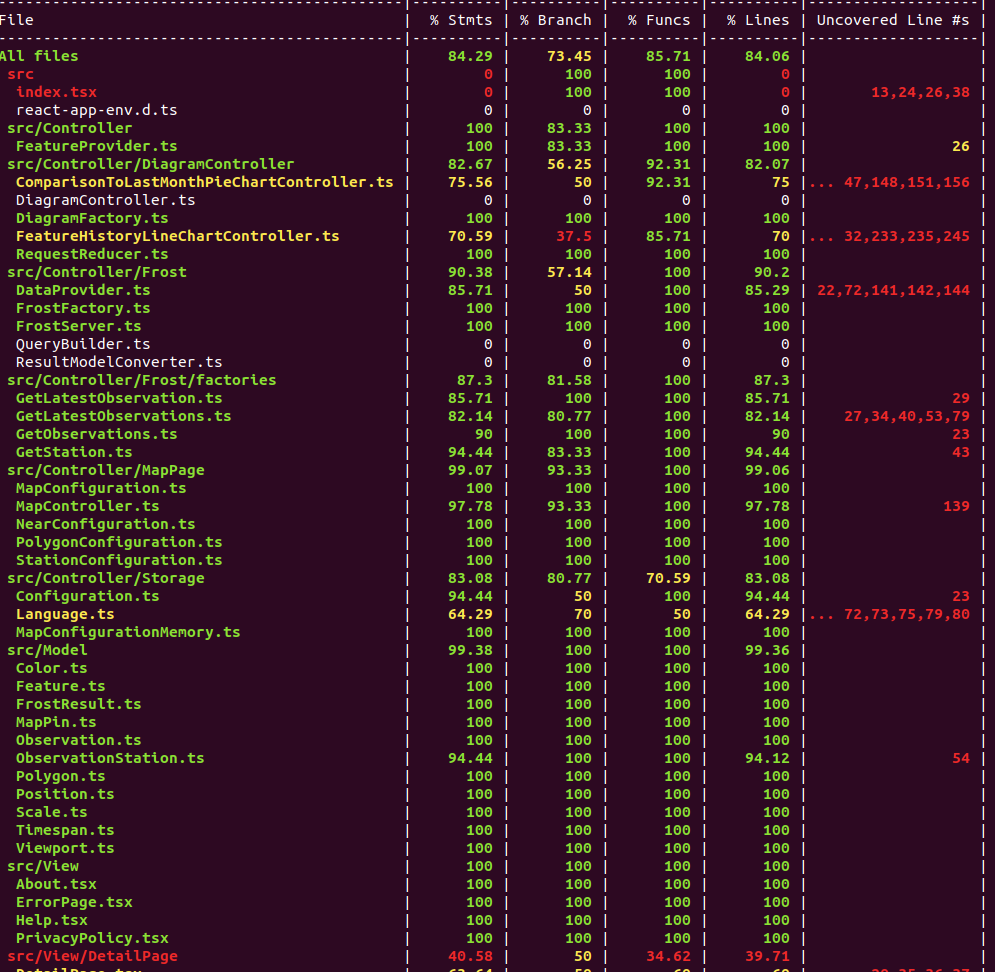
\includegraphics[width=1\linewidth]{figures/Testcoverage1.png}\par\vspace{1cm}
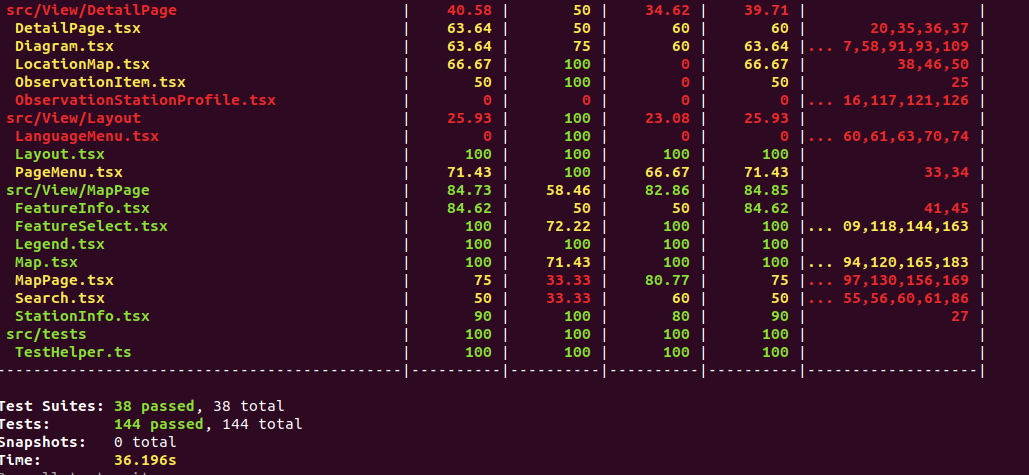
\includegraphics[width=1\linewidth]{figures/Testcoverage2.png}\par\vspace{1cm}

\subsection{Bugs and Fixes}

Da diee Webanwendung rein frontend ist, passiert wenig im Hintergrund, ohne dass man es auf der Benutzeroberfläche sofort merken würde. Deshalb dienen die meisten Unit-Tests als Sicherheitstests um hauptsächlich Kleinigkeiten und Sonderfälle zu testen. 

\begin{Bug}{Karte auszoomen}
    \textbf{Problem}\\
    Wenn die größtmöglichen Koordinaten erreicht werden, die Webanwendung stürzt ab.\\
    \linebreak
    \textbf{Lösung}\\
    Wir haben eine Grenze für das maximale Auszoomen gesetzt.\\
\end{Bug}


